%!TEX TS-program = xelatex
\documentclass[]{friggeri-cv}
\usepackage{afterpage}
\usepackage{hyperref}
\usepackage{color}
\usepackage{xcolor}
\hypersetup{
    pdftitle={},
    pdfauthor={},
    pdfsubject={},
    pdfkeywords={},
    colorlinks=false,       % no lik border color
   allbordercolors=white    % white border color for all
}
\addbibresource{bibliography.bib}
\RequirePackage{xcolor}
\definecolor{pblue}{HTML}{0395DE}

\begin{document}
\header{Tiago O.}{ de Farias}
      {Analista de Sistemas PHP}
      
% Fake text to add separator      
\fcolorbox{white}{gray}{\parbox{\dimexpr\textwidth-2\fboxsep-2\fboxrule}{%
.....
}}

% In the aside, each new line forces a line break
\begin{aside}
  \section{Endereço}  	
    Rua Doutor José Bento Corrêa, 545
    Bairro Protásio Alves,
    CEP: 91450-030
    Rio Grande do Sul, Porto Alegre
    ~
  \section{Telefone}
    51 9292 2705
    51 3018 1864
    ~
  \section{E-mail}
    \href{mailto:tiago.farias.poa@gmail.com}{\textbf{tiago.farias.poa@}\\gmail.com}
    ~
  \section{Web \& Git}
    \href{https://github.com/tofarias}{github.com/tofarias}
    \href{https://bitbucket.org/tiagofarias}{bitbucket.org/tiagofarias}
    \href{https://tiagoodefarias.wordpress.com/}{tiagoodefarias.wordpress}
    \href{https://www.facebook.com/groups/laravelrgs}{facebook.com/laravelrgs}
    ~
  \section{Programação}
    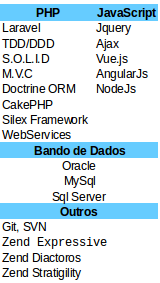
\includegraphics[scale=0.62]{img/techinical-skills.png}
    ~
  \section{Sistemas Operacionais}
    \textbf{GNU/Linux}
\includegraphics[scale=0.40]{img/4stars.png}
    \textbf{Windows}
\includegraphics[scale=0.40]{img/3stars.png}
    ~
  \section{Personal Skills}
    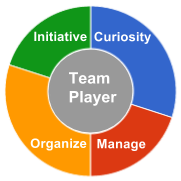
\includegraphics[scale=0.62]{img/personal.png}
    ~
\end{aside}

\section{Formação}
\begin{entrylist}
  \entry
    {2014 - 2016}
    {Pós-Graduação: Sist. de Informação com Métodos Ágeis}
    {UniRitter}
    {Tópicos principais: Práticas de Desenvolvimento Ágil, Design Patterns, Smells e Refatoring, Arquiteturas para Web, Testes Ágeis de Software, Gerência de Projetos, Agile Coaching e Mentoring.\\
    \emph{Título do Artigo: "Aplicação de Domain-Driven Design no Gerenciamento de
GRU de Cronotacógrafo no Inmetro/RS".}\\
    \emph{Orientador: M.e. Guilherme Silva de Lacerda.}\\
    Endereço: Rua Orfanotrófio, 555 - Alto Petrópolis, Porto Alegre/RS\\}
  \entry
    {2010 - 2013}
    {Graduação: Análise e Desenvolvimento de Sistemas}
    {Faculdades QI}
    {Tópicos principais: Serviços para Web, Gestão de Projetos, Segurança de Software, Engenharia de Software, Desenvolvimento Java O.O.\\
    Endereço: Av. Julho de Castilhos, 435 - Centro, Porto Alegre/RS\\}
    
  \entry
    {2008 - 2010}
    {Técnico: Informática.}
    {Faculdades QI}
    {Endereço: Av. Assis Brasil, 3312 - Porto Alegre/RS}
\end{entrylist}

\section{Experiência}
\begin{entrylist}
  \entry
    {03/2015 - hoje}
    {Programador}
    {Advanced IT}
    {Alocado no cliente Inmetro. Atua principalmente com a linguagem PHP (CakePHP) e banco de dados Oracle no projeto Cronotacógrafo. Realiza desde o levantamento de requisitos através de entrevistas com usuário até a análise de impacto juntamente com os administradores de banco de dados.\\}
  \entry
    {08/2013 - 03/2015}
    {Analista de Sistemas}
    {Construtora Pelotense}
    {Atuou no desenvolvimento de sistema web interno que tem por objetivo gerenciar contratos e faturas das obras. O módulo de faturas é carregado com informações da base de dados (SQL Server) gerenciada pelo sistema da TOTVS: RM e Fluxos. Desenvolveu com PHP (Laravel), TDD, Git, em ambiente linux juntamente com banco de dados MySql.\\}
    \entry
    {01/2013 - 08/2013}
    {Programador de Computador}
    {Constat}
    {Atuou principalemten com a linguagem PHP. Responsável por desenvolver soluções para o produto Qualitor e seus módulos. Realizava Análise de requisitos, documentação de projeto, desenvolvimento com TDD e gerência de configuração.\\}
    \entry
    {05/2012 - 12/2012}
    {Técnico em Informática}
    {EMATER/ASCAR}
    {Ingressou mediante concurso público, atuando na manutenção de computadores nos escritórios municipais. Eventualmente desenvolveu programas em Java para auxiliar nas demandas do setor.\\}
    \entry    
    {04/2011 - 05/2012}
    {Programador de Computador}
    {CWI Software}
    { Ingressou em abril/2011 no projeto “Crescer” da empresa CWI Software que ocorreu em São Leopoldo, o treinamento com duração de 2 meses envolveu as seguintes tecnologias: SQL Server 2008, ASP.Net, C\#, Java Web. Com o término do projeto “Crescer” continuou na empresa como estagiário trabalhando no suporte técnico na sede São Leopoldo com PHP/Zend Framework para o cliente “TUV Rheinland” e CodeIgniter para o cliente Terra, foi transferido para a unidade em Porto Alegre ingressando no projeto do cliente “Odebrecht”,
utilizando as tecnologias dotNet MVC e PL/SQL, após ingressou na equipe de desenvolvimento para o cliente SENAC/RS no projeto para desenvolver a intranet da empresa utilizando dotNET MVC e SqlServer
2008.\\}
\end{entrylist}



\section{Certifications}
\begin{entrylist}
  \entry
    {02/2013}
    {Intro to Computer Science}
    {Udacity. E-learning}
    {\emph{Building a Python Search Engine}}
\end{entrylist}

\newpage

\begin{aside}
~
~
~
  \section{Places Lived}
    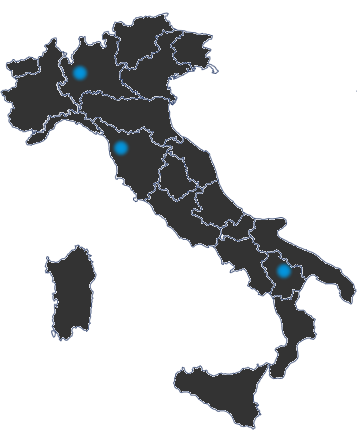
\includegraphics[scale=0.25]{img/italia.png}
    ~
  \section{Languages}
    \textbf{Italian}
\includegraphics[scale=0.40]{img/5stars.png}
    \textbf{English}
\includegraphics[scale=0.40]{img/4stars.png}
\end{aside}

\section{Publications}
C. Benedetto, E. Mingozzi, C. Vallati\\
\textbf{A Handoff Algorithm based on Link Quality Prediction for Mass Transit Wireless Mesh Networks}\\
\emph{Proceedings of the 18th IEEE Symposium on Computers and Communications (ISCC 2013), Split, Croatia, July 7-10, 2013}
\\
\section{Other Info}
For the Italian job market:\\
\emph{Si autorizza il trattamento delle informazioni contenute nel curriculum in conformità alle disposizioni previste dal d.lgs. 196/2003. Si dichiara altresì di essere consapevole che, in caso di dichiarazioni non veritiere, si è passibili di sanzioni penali ai sensi del DPR 445/00 oltre alla revoca dei benefici eventualmente percepiti.}
\\
\begin{flushleft}
\emph{January 14th, 2014}
\end{flushleft}
\begin{flushright}
\emph{Carmine Benedetto}
\end{flushright}

%%% This piece of code has been commented by Karol Kozioł due to biblatex errors. 
% 
%\printbibsection{article}{article in peer-reviewed journal}
%\begin{refsection}
%  \nocite{*}
%  \printbibliography[sorting=chronological, type=inproceedings, title={international peer-reviewed conferences/proceedings}, notkeyword={france}, heading=subbibliography]
%\end{refsection}
%\begin{refsection}
%  \nocite{*}
%  \printbibliography[sorting=chronological, type=inproceedings, title={local peer-reviewed conferences/proceedings}, keyword={france}, heading=subbibliography]
%\end{refsection}
%\printbibsection{misc}{other publications}
%\printbibsection{report}{research reports}

\end{document}
